\documentclass[preview]{standalone}
\usepackage{amssymb}
\usepackage{mathtools}


\begin{document}


% ============================== 0001 Algorithm 3103 ================================
\subsection[The sum of integers in a list.]{
    \color{section} Algorithm 1. \color{black} The sum of integers in a list.
}
\vspace{-1\baselineskip}
\documentclass[preview]{standalone}
\usepackage{xcolor}
\usepackage[noend]{algpseudocode}


\newcommand{\pluseq}{\mathrel{+}=}


\begin{document}
    \begin{algorithmic}[0]
        \Statex \color{white} x \color{black}
        \Function{sum}{$\rho_1, \rho_2, \dots, \rho_\epsilon$: list of integers}
            \State $\phi \gets 0$
            \For{$\iota \gets 1, \epsilon$}
                \State $\phi \pluseq \rho_\iota$
            \EndFor
            \State \Return{$\phi$}
        \EndFunction        
    \end{algorithmic}

\end{document}
\begin{center}
    \lstinputlisting[language=Python, title=\textbf{\color{darkgray}Python}]{../resources/Python/3.1.algorithms/3103.py}
\end{center}
\vspace{.3\baselineskip}
\begin{center}
    \lstinputlisting[language=Java, title=\textbf{\color{darkgray}Java}, firstline=9, lastline=16]{../resources/Java/3.1.algorithms/j3103.java}
\end{center}

\pagebreak


% ============================== 0002 Algorithm 3104 ================================
\begin{figure}[!h]
    \centering
    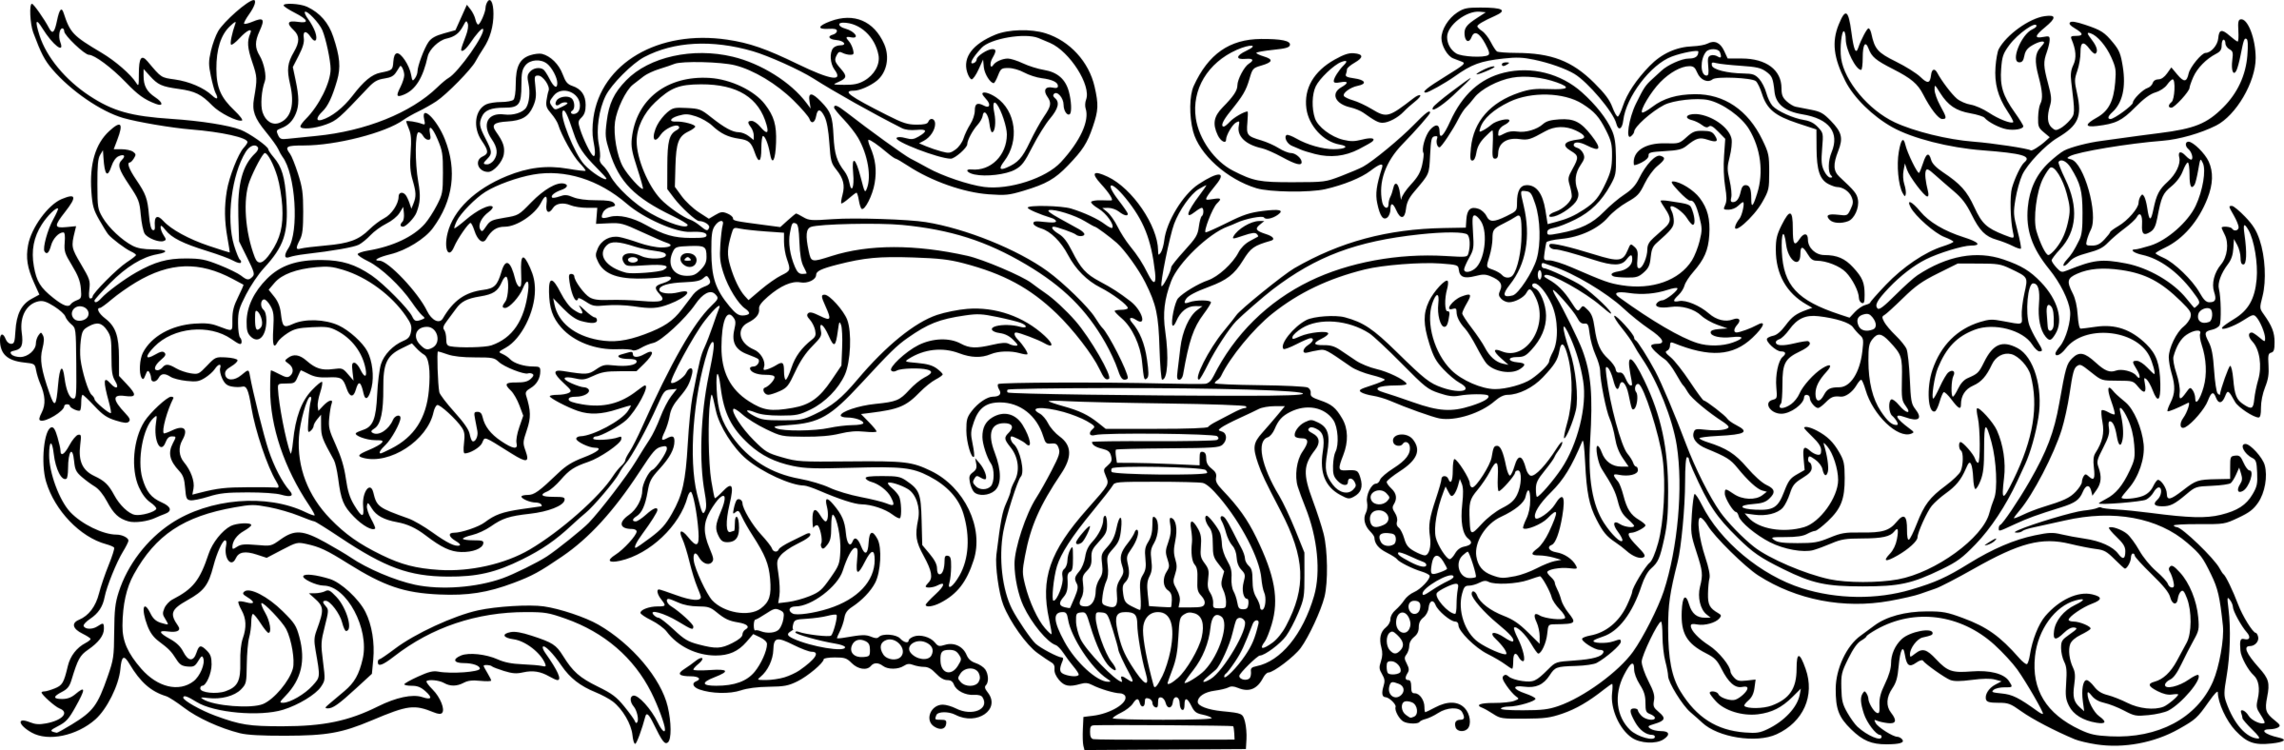
\includegraphics[width=14cm]{../resources/jpg/3.1.algorithms/border1.png}
\end{figure}
\subsection[Max adjacent list entry difference.]{
    \color{section} Algorithm 2. \color{black} Max adjacent list entry difference.
}
\vspace{-1\baselineskip}
\documentclass[preview]{standalone}
\usepackage{xcolor}
\usepackage[noend]{algpseudocode}

\begin{document}
    
    \begin{algorithmic}[0]
        
        \Statex \color{white} x \color{black}
        \Function{max difference}{$\rho_1, \rho_2, \dots, \rho_\epsilon$: list of integers}
        \State $\mu \gets 0$
        \For{$\iota = 2, \epsilon$}
            \State $\sigma = \rho_\iota - \rho_{\iota-1}$
            \If {$\mu < \sigma$}
                \State $\mu = \sigma$
            \EndIf
        \EndFor
        \State \Return{$\mu$}
        \EndFunction

    \end{algorithmic}

\end{document}
\begin{center}
    \lstinputlisting[language=Python, title=\textbf{\color{darkgray}Python}]{../resources/Python/3.1.algorithms/3104.py}
\end{center}
\begin{center}
    \lstinputlisting[language=Java, title=\textbf{\color{darkgray}Java}, firstline=9, lastline=19]{../resources/Java/3.1.algorithms/j3104.java}
\end{center}
\pagebreak


% ============================== 0003 Algorithm 3105 ================================
\begin{figure}[!h]
    \centering
    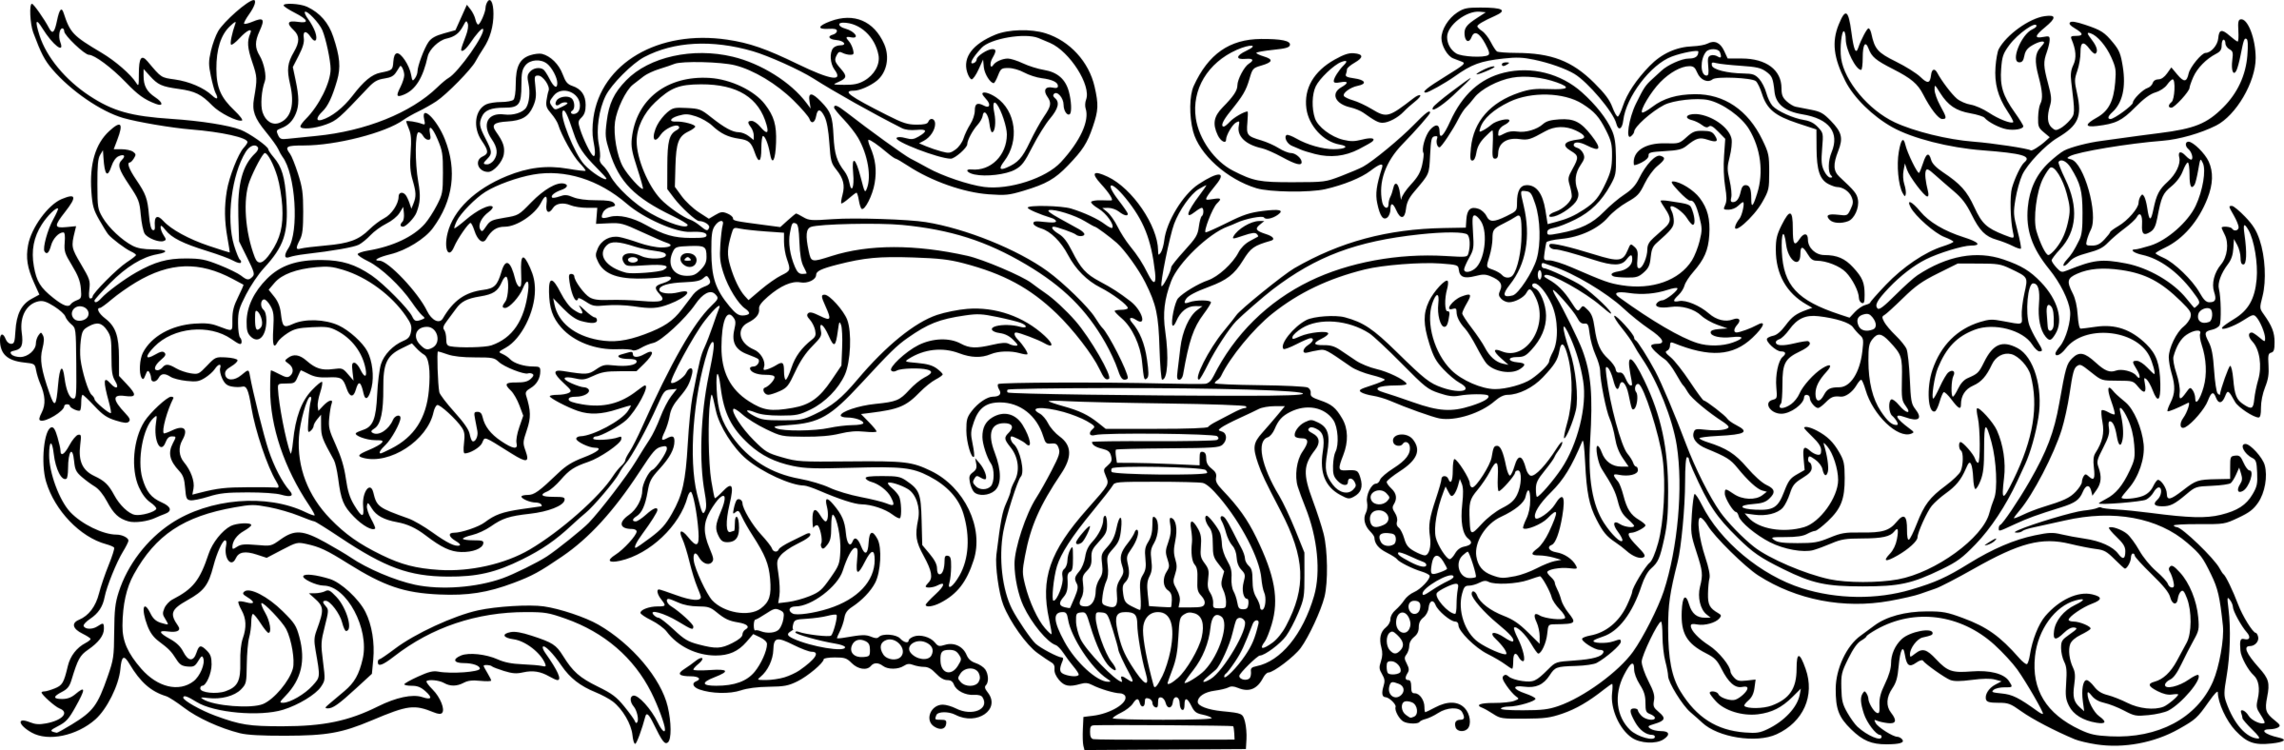
\includegraphics[width=14cm]{../resources/jpg/3.1.algorithms/border1.png}
\end{figure}
\subsection[Find duplicate list entries.]{
    \color{section} Algorithm 3. \color{black} Find duplicate list entries.
}
\vspace{-1\baselineskip}
\documentclass[preview]{standalone}
\usepackage{xcolor}
\usepackage[noend]{algpseudocode}
\usepackage{amssymb}


\begin{document}


\begin{algorithmic}[0]
    
    \Statex \color{white} x \color{black}
    \Function{duplicates}{$\rho_1, \rho_2, \dots, \rho_\epsilon$: integers in nondecreasing order}
    \State $\phi \gets \varnothing$
    \For{$\iota = 1, \epsilon-1$}
        \If {$\rho_\iota = \rho_{\iota+1}$}
            \State $\phi \gets \phi \cup \{\rho_{\iota+1}\}$
        \EndIf
    \EndFor
    \State \Return{$\phi$} 
    \EndFunction
    
\end{algorithmic}


\end{document}
\begin{center}
    \lstinputlisting[language=Python, title=\textbf{\color{darkgray}Python}]{../resources/Python/3.1.algorithms/3105.py}
\end{center}
\begin{center}
    \lstinputlisting[language=Java, title=\textbf{\color{darkgray}Java}, firstline=11, lastline=21]{../resources/Java/3.1.algorithms/j3105.java}
\end{center}
\pagebreak


% ============================== 0004 Algorithm 3106 ================================
\begin{figure}[!h]
    \centering
    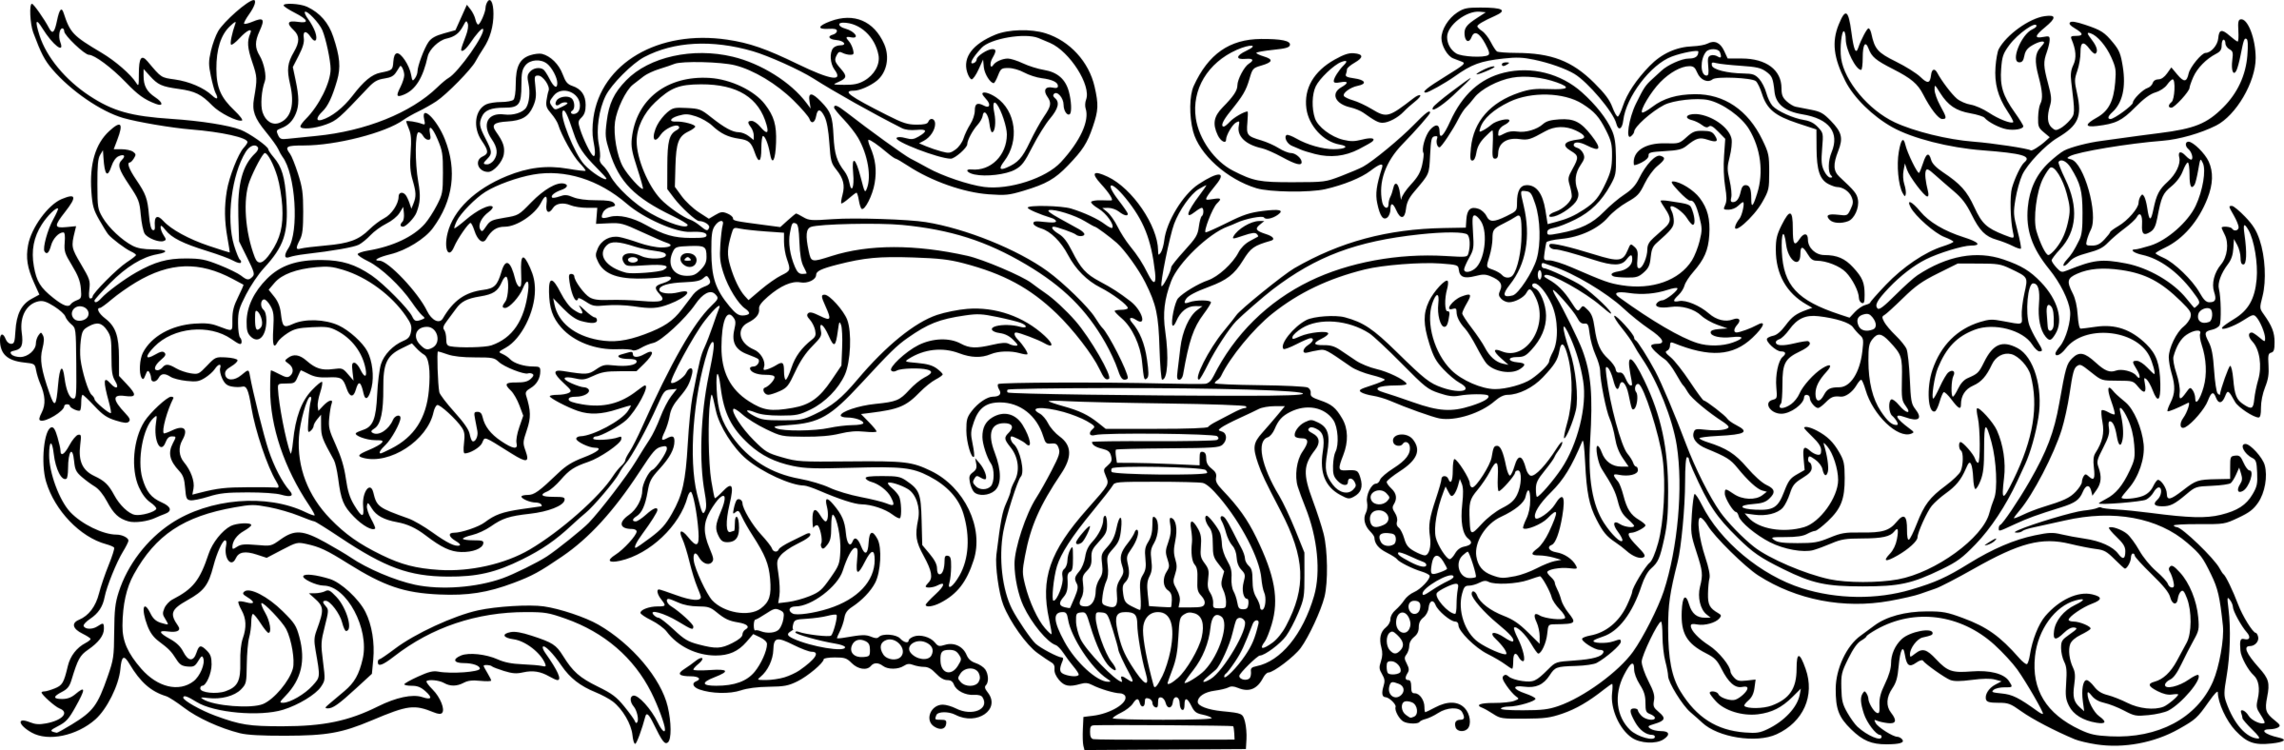
\includegraphics[width=14cm]{../resources/jpg/3.1.algorithms/border1.png}
\end{figure}
\subsection[Count negative valued list entries.]{
    \color{section} Algorithm 4. \color{black} Count negative valued list entries.
}
\vspace{-1\baselineskip}
\documentclass[preview]{standalone}
\usepackage{xcolor}
\usepackage[noend]{algpseudocode}


\newcommand{\pluseq}{\mathrel{+}=}


\begin{document}

\begin{algorithmic}[0]
    \Statex \color{white} x \color{black}
    \Function{negatives}{$\rho_1, \rho_2, \dots, \rho_\epsilon$: list of integers}
    \State $\phi \gets 0$
    \For{$\iota = 1, \epsilon$}
        \If {$\rho_\iota < 0$}
            \State $\phi \pluseq 1$
        \EndIf
    \EndFor
    \State \Return{$\phi$}
    \EndFunction
    
\end{algorithmic}

\end{document}
\vspace{1\baselineskip}
\begin{center}
    \lstinputlisting[language=Python, title=\textbf{\color{darkgray}Python}]{../resources/Python/3.1.algorithms/3106.py}
\end{center}
\vspace{1\baselineskip}
\begin{center}
    \lstinputlisting[language=Java, title=\textbf{\color{darkgray}Java}, firstline=11, lastline=20]{../resources/Java/3.1.algorithms/j3106.java}
\end{center}
\pagebreak


% ============================== 0005 Algorithm 3107 ================================
\begin{figure}[!h]
    \centering
    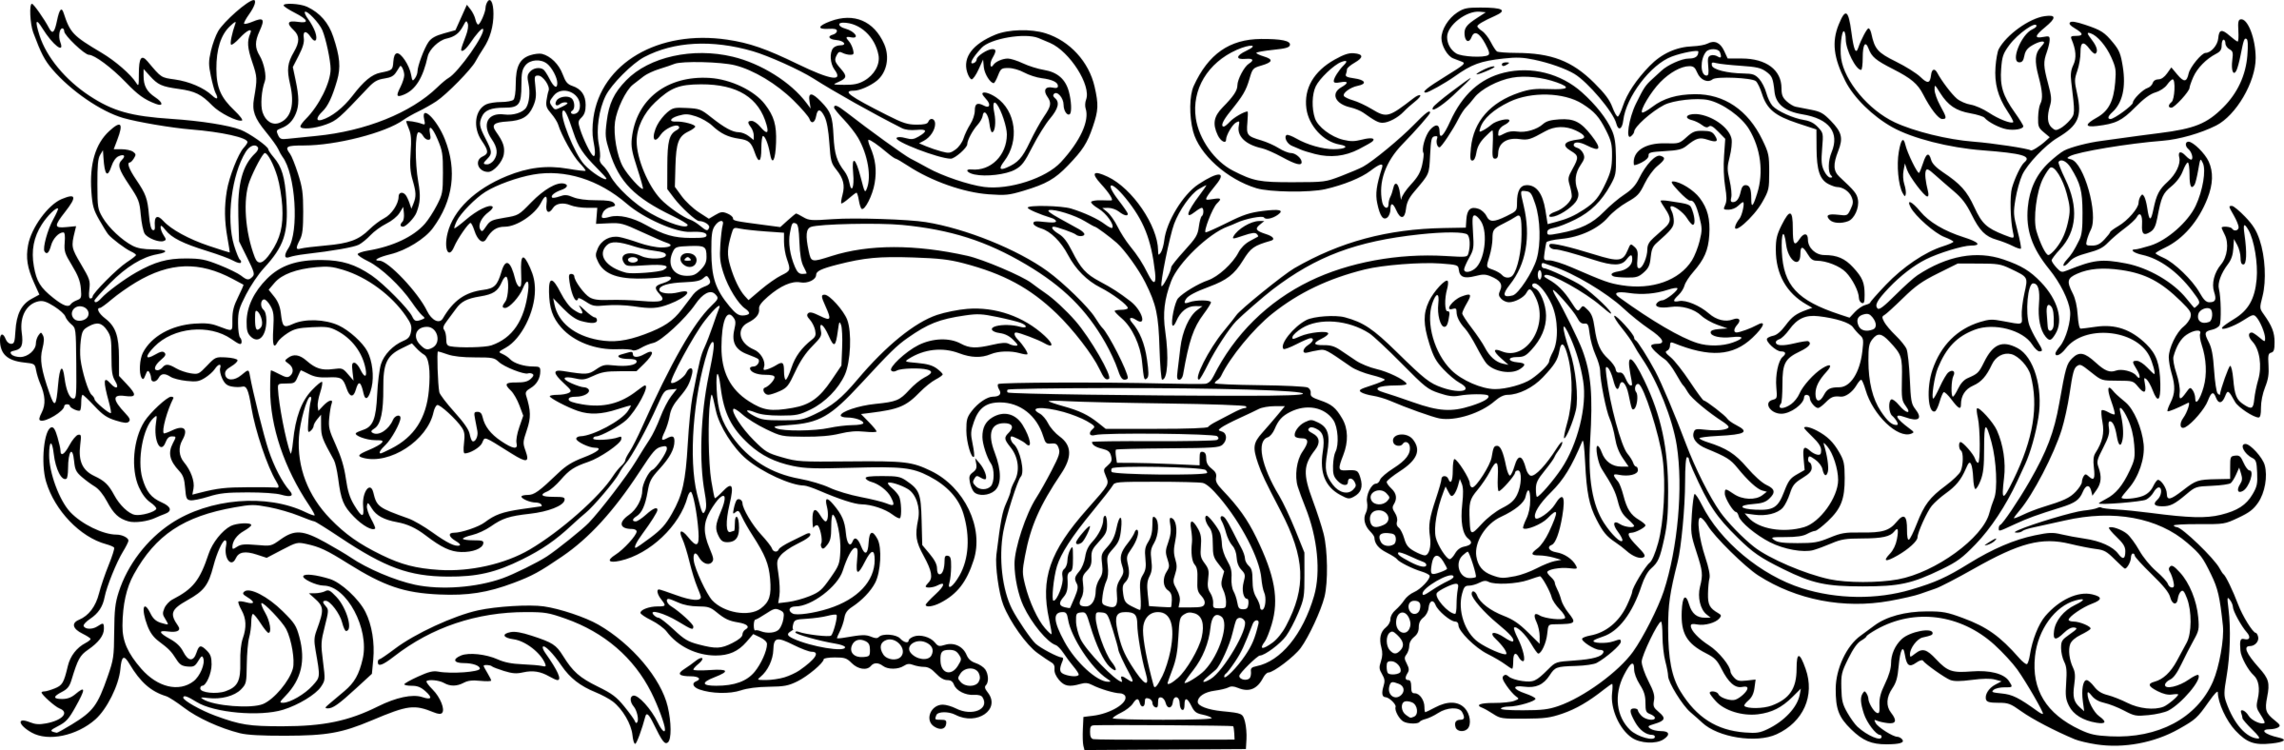
\includegraphics[width=14cm]{../resources/jpg/3.1.algorithms/border1.png}
\end{figure}
\subsection[Find the last even list entry.]{
    \color{section} Algorithm 5. \color{black} Find the last even list entry.
}
\vspace{-1\baselineskip}
\documentclass[preview]{standalone}
\usepackage{xcolor}
\usepackage[noend]{algpseudocode}
\usepackage{mathtools}


\DeclareMathOperator*{\nullspace}{null}


\begin{document}

    \begin{algorithmic}[0]
        \Statex \color{white} x \color{black}
        \Function{last even}{$\rho_1, \rho_2, \dots, \rho_\epsilon$: list of integers}
        \State $\phi \gets \nullspace$
        \For{$\iota = 1, \epsilon$}
            \If {$\lnot \big [ \rho_\iota \langle $mod $ 2 \rangle \big ]$}
                \State $\phi \gets \iota$
            \EndIf
        \EndFor
        \State \Return{$\phi$}
        \color{lightgray} \Comment{returns $\nullspace$ if every integer $\rho_\iota$ is odd}
        \color{black}
        \EndFunction
    
    \end{algorithmic}

\end{document}
\vspace{1\baselineskip}
\begin{center}
    \lstinputlisting[language=Python, title=\textbf{\color{darkgray}Python}]{../resources/Python/3.1.algorithms/3107.py}
\end{center}
\vspace{1\baselineskip}
\begin{center}
    \lstinputlisting[language=Java, title=\textbf{\color{darkgray}Java}, firstline=11, lastline=20]{../resources/Java/3.1.algorithms/j3107.java}
\end{center}
\pagebreak


% ============================== 0006 Algorithm 3108 ================================
\begin{figure}[!h]
    \centering
    
\includegraphics[width=14cm]{../resources/jpg/3.1.algorithms/border2.jpg}
\end{figure}
\subsection[Find the largest even list entry.]{
    \color{section} Algorithm 6. \color{black} Find the largest even list entry.
}
\vspace{-1\baselineskip}
\documentclass[preview]{standalone}
\usepackage{xcolor}
\usepackage[noend]{algpseudocode}
\usepackage{mathtools}


\DeclareMathOperator*{\nullspace}{null}


\begin{document}
    
\begin{algorithmic}[0]
    \Statex \color{white} x \color{black}
    \Function{largest even}{$\rho_1, \rho_2, \dots, \rho_\epsilon$: list of integers}
    \State $\phi \gets \nullspace$
    \For{$\iota = 1, \epsilon$}
        \If {$\lnot \big [ \rho_\iota \langle $mod $2 \rangle \big ]$}
            \If {$\langle \phi = \nullspace \rangle \lor \langle \rho_\iota > \rho_{\phi} \rangle$}
                \State $\phi \gets \iota$
            \EndIf
        \EndIf
    \EndFor
    \State \Return{$\phi$}
    \color{lightgray}\Comment{returns null if every integer is odd} \color{black}
    \EndFunction
    
\end{algorithmic}

\end{document}
\vspace{1\baselineskip}
\begin{center}
    \lstinputlisting[language=Python, title=\textbf{\color{darkgray}Python}]{../resources/Python/3.1.algorithms/3108.py}
\end{center}
\vspace{1\baselineskip}
\begin{center}
    \lstinputlisting[language=Java, title=\textbf{\color{darkgray}Java}, firstline=11, lastline=23]{../resources/Java/3.1.algorithms/j3108.java}
\end{center}
\pagebreak


% ============================== 0007 Algorithm 3109 ================================
\begin{figure}[!h]
    \centering
    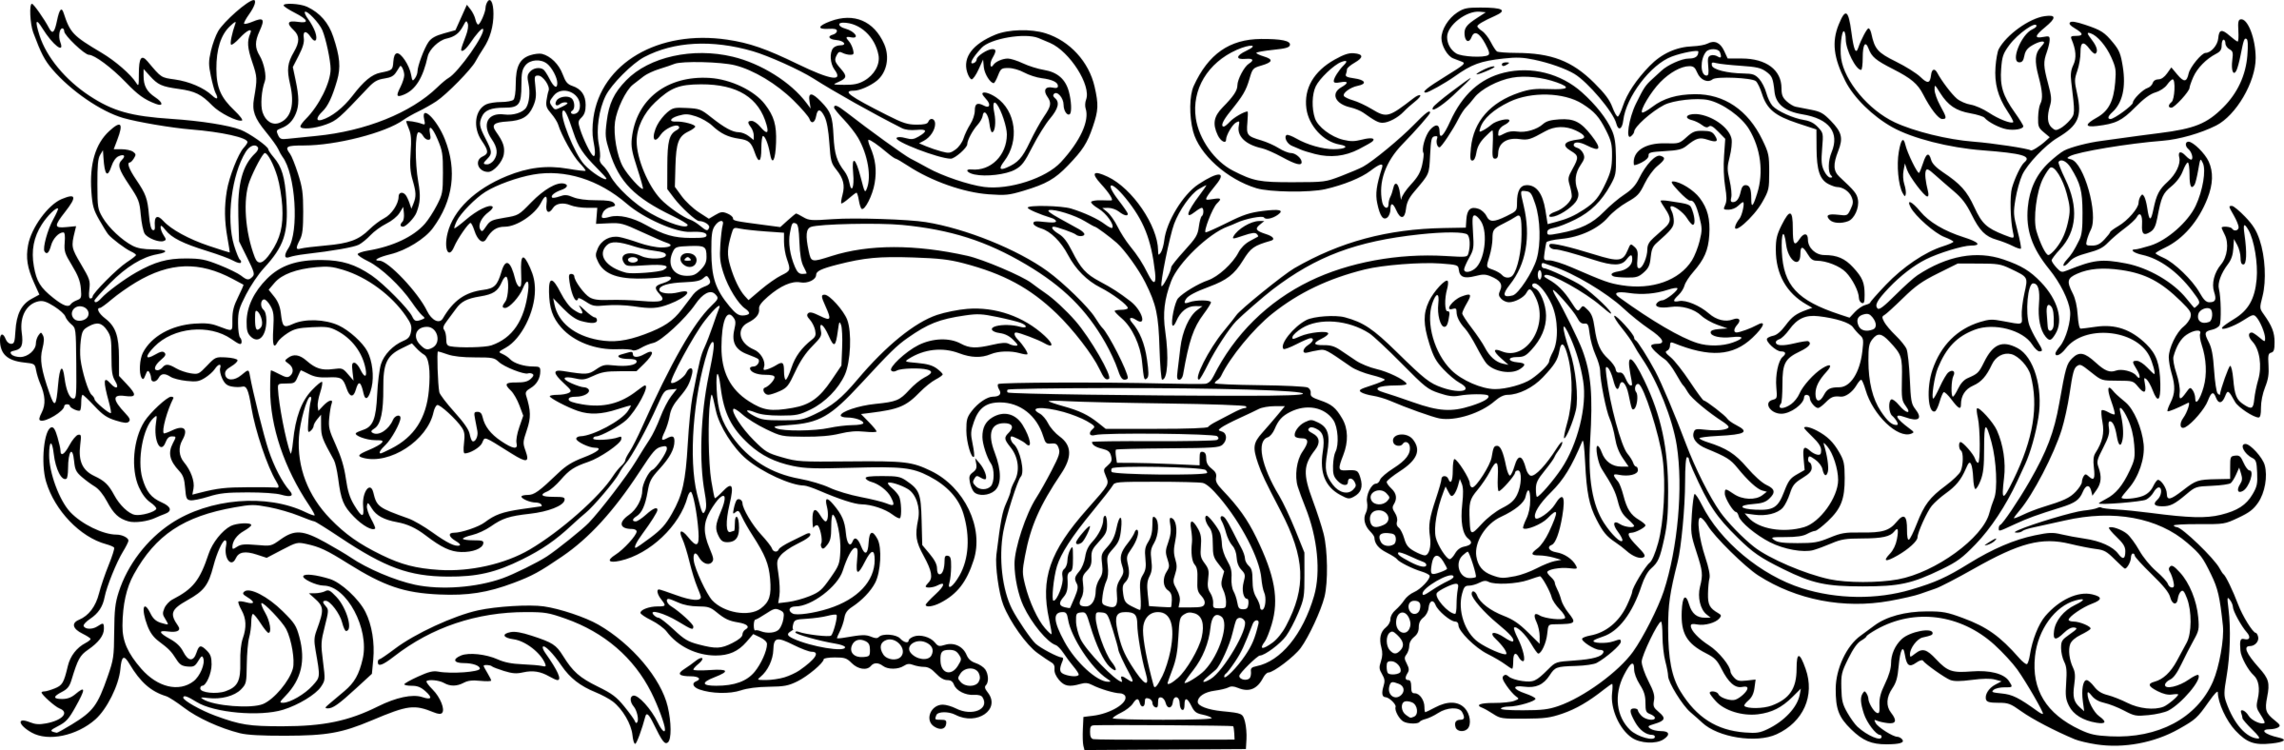
\includegraphics[width=14cm]{../resources/jpg/3.1.algorithms/border1.png}
\end{figure}
\subsection[Palindrome strings of characters.]{
    \color{section} Algorithm 7. \color{black} Palindrome strings of characters.
}
\vspace{-1\baselineskip}
\documentclass[preview]{standalone}
\usepackage{xcolor}
\usepackage[noend]{algpseudocode}


\begin{document}

    \begin{center}
        \text{\emph{Determine whether a string is a palindrome.}}
    \end{center}

    \begin{algorithmic}[0]
        \Statex \color{white} x \color{black}
        \Function{palindrome}{$\rho_1, \rho_2, \dots, \rho_\epsilon$: string of characters}
        \For{$\iota = 1, \big \lfloor \frac{\epsilon}{2} \big \rfloor$}
            \If {$\rho_\iota \ne \rho_{\langle \epsilon+1 \rangle - \iota}$}
                \State \Return{$\bot$}
            \EndIf
        \EndFor
        \State \Return{$\top$}
        \color{lightgray} \Comment{all of the characters matched} \color{black}
        \EndFunction
    \end{algorithmic}
\end{document}
\vspace{1\baselineskip}
\begin{center}
    \lstinputlisting[language=Python, title=\textbf{\color{darkgray}Python}]{../resources/Python/3.1.algorithms/3109.py}
\end{center}
\vspace{0\baselineskip}
\begin{center}
    \lstinputlisting[language=Java, title=\textbf{\color{darkgray}Java}, firstline=11, lastline=21]{../resources/Java/3.1.algorithms/j3109.java}
\end{center}
\pagebreak


% ============================= 0008 Algorithm 3110 =================================
\subsection[Compute beta to the power of lambda.]{
    \color{section} Algorithm 8. \color{black} Compute \bm{$\beta^\lambda$}
}
\vspace{-1\baselineskip}
\documentclass[preview]{standalone}
\usepackage{xcolor}
\usepackage[noend]{algpseudocode}


\newcommand{\minuseq}{\mathrel{-}=}


\begin{document}
    
    \begin{algorithmic}[0]
        \Statex \color{white} x \color{black}
        \Function{power}{$\lambda$: integer; $\beta$: real number}
    
        \State $\epsilon \gets \big|\lambda  \big|$
        \State $\rho \gets 1$
    
        \While{$\epsilon > 0$} 
        \color{lightgray}\Comment {multiply $\beta$ by itself $\big|\lambda\big|$ times} \color{black}
            \State $\rho \gets \rho \times \beta$
            \State $\epsilon \minuseq 1$
        \EndWhile
        \If {$\lambda < 0$} 
        \color{lightgray} \Comment{$\lambda$ is negative so get the inverse} \color{black}
            \State $\rho \gets \frac{1}{\rho}$
        \EndIf
        \State \Return{$\rho$}
        \EndFunction
    
    \end{algorithmic}

\end{document}
\vspace{1\baselineskip}
\begin{center}
    \lstinputlisting[language=Python, title=\textbf{\color{darkgray}Python}]{../resources/Python/3.1.algorithms/3110.py}
\end{center}
\vspace{1\baselineskip}
\begin{center}
    \lstinputlisting[language=Java, title=\textbf{\color{darkgray}Java}\text{\newline}, firstline=12, lastline=24]{../resources/Java/3.1.algorithms/j3110.java}
\end{center}
\pagebreak


% ============================= 0009 Algorithm 3111 =================================
\begin{figure}[!h]
    \centering
    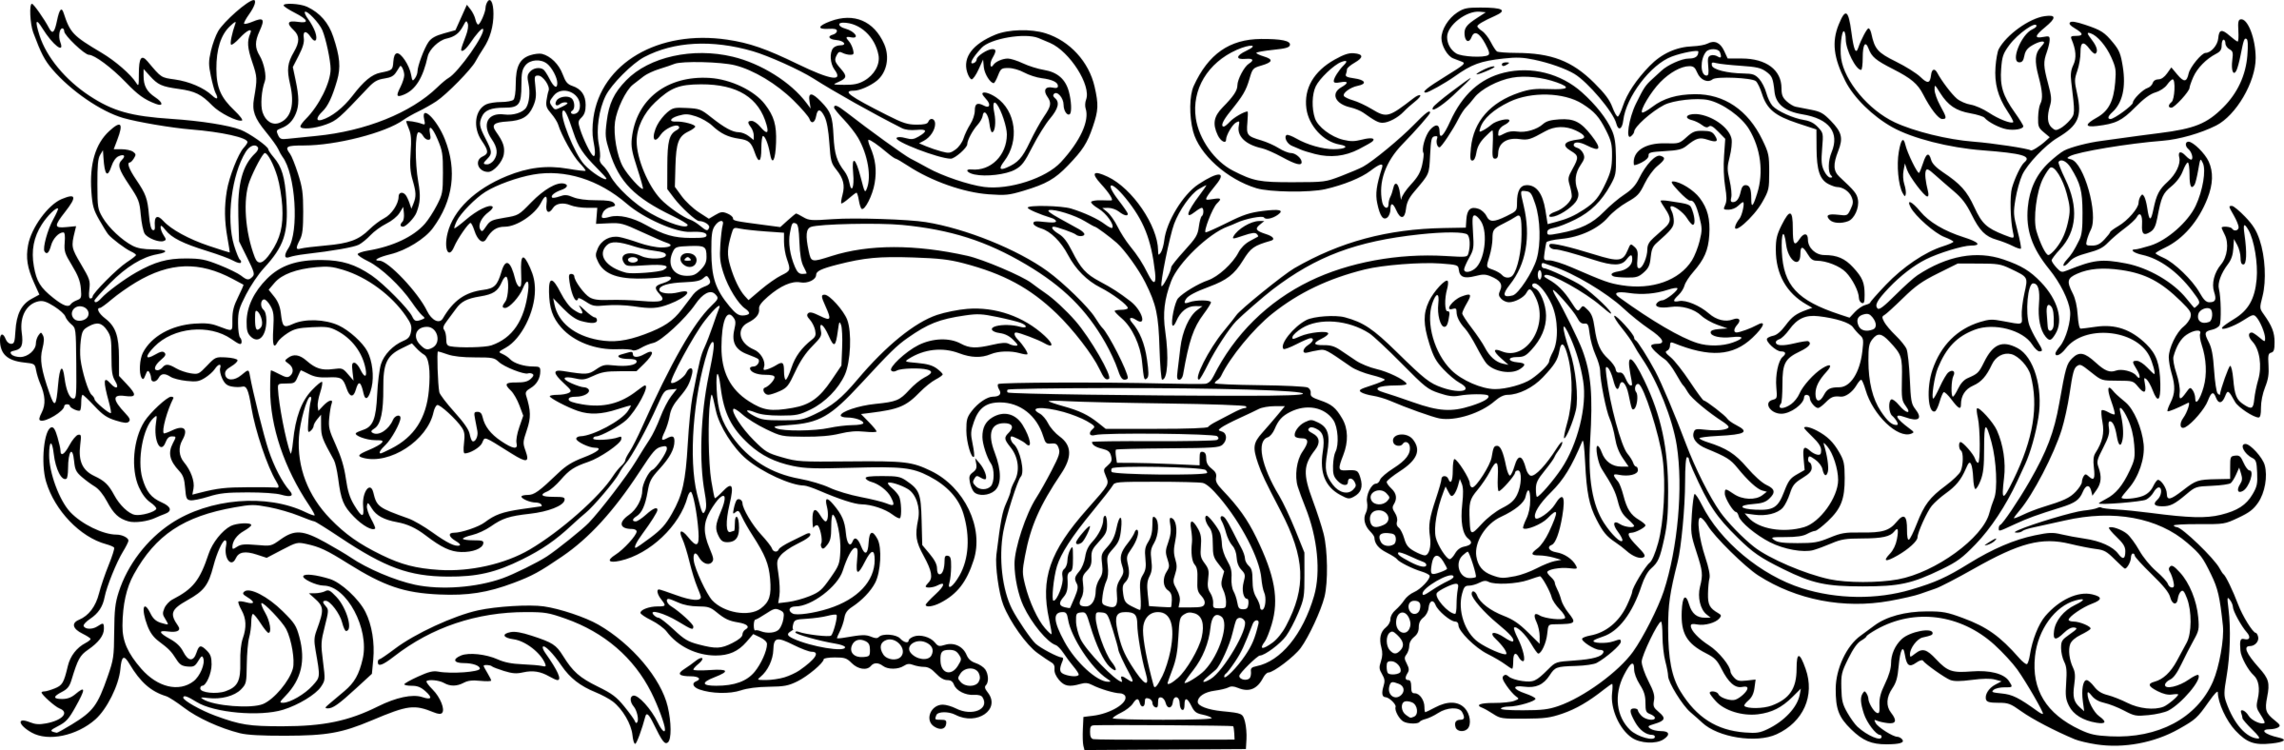
\includegraphics[width=14cm]{../resources/jpg/3.1.algorithms/border1.png}
\end{figure}
\subsection[Swap lambda with iota.]{
    \color{section} Algorithm 9. \color{black} Swap \bm{$\lambda$} with \bm{$\iota$}.
}
\vspace{-1\baselineskip}
\documentclass[preview]{standalone}
\usepackage{xcolor}
\usepackage[noend]{algpseudocode}


\begin{document}
    
    \begin{algorithmic}[0]
        \Statex \color{white} x \color{black}
        \Function{swap}{$\lambda$: object; $\iota$: object}
    
        \State $\tau \gets \lambda$
        \State $\lambda \gets \iota$
        \State $\iota \gets \tau$

        \State \Return{$\lambda, \iota$}
        \EndFunction
    
    \end{algorithmic}

\end{document}
\vspace{1\baselineskip}
\begin{center}
    \lstinputlisting[language=Python, title=\textbf{\color{darkgray}Python}]{../resources/Python/3.1.algorithms/3111.py}
\end{center}
\vspace{.7\baselineskip}
\begin{center}
    \lstinputlisting[language=Java, title=\textbf{\color{darkgray}Java}, firstline=13, lastline=21]{../resources/Java/3.1.algorithms/j3111.java}
\end{center}
\pagebreak


% ============================= 0010 Algorithm 3115 =================================
\begin{figure}[!h]
    \centering
    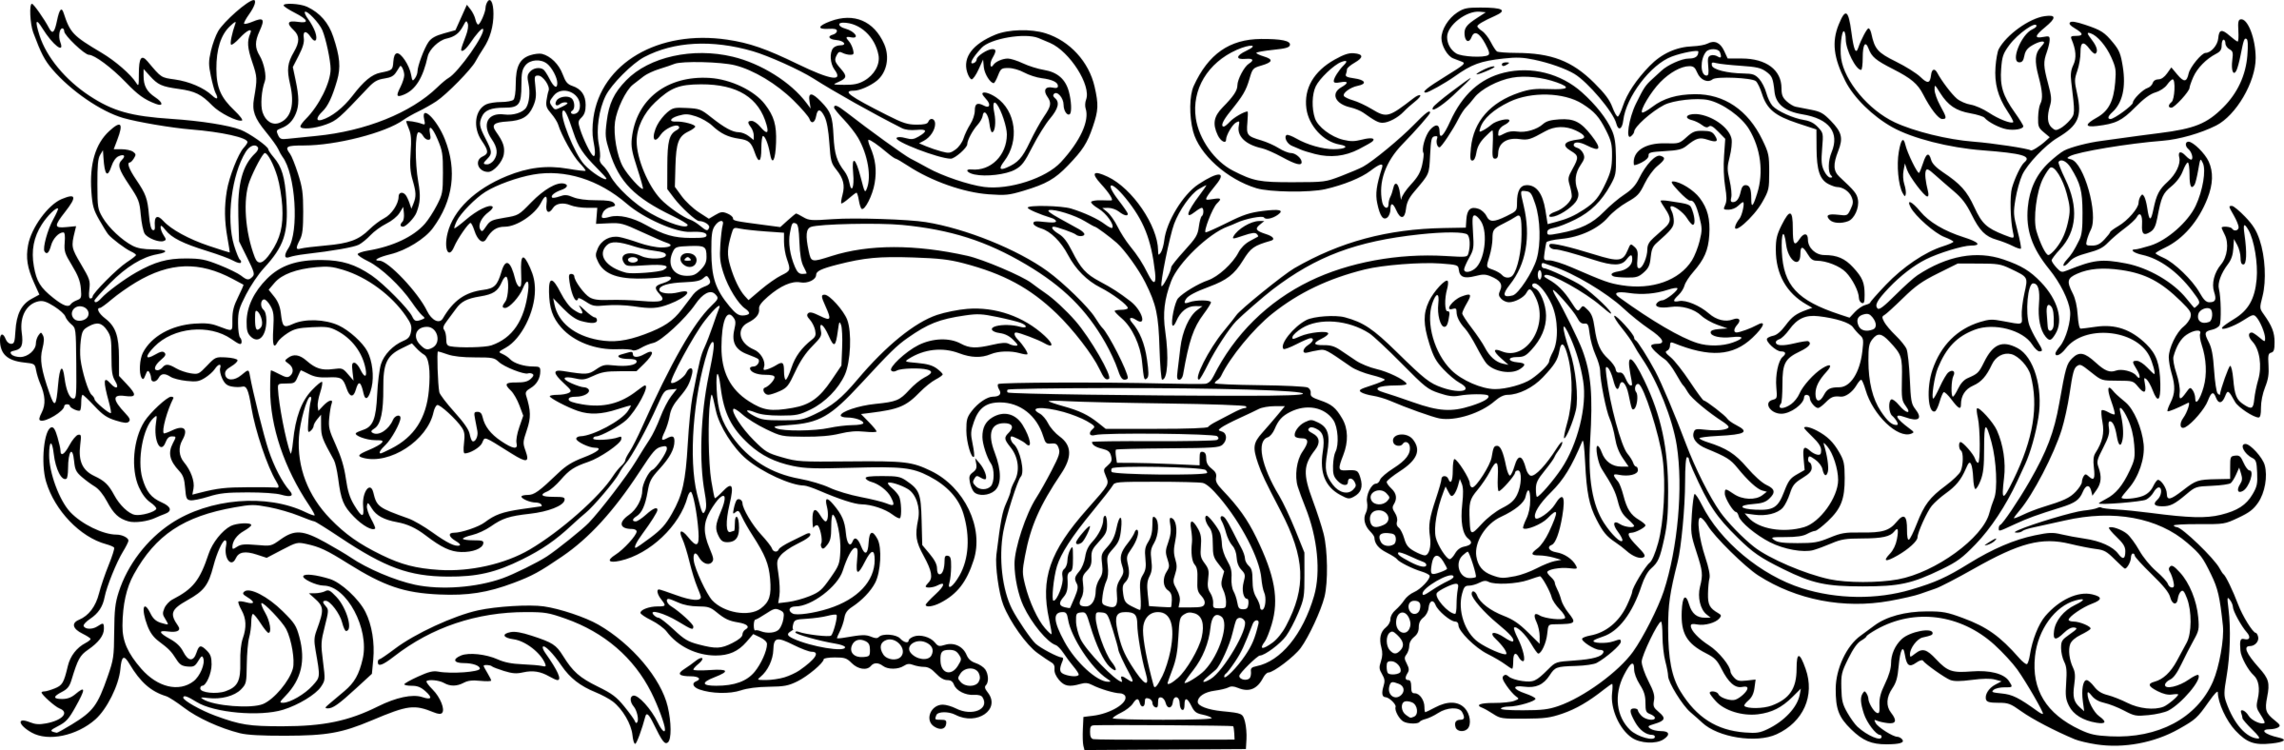
\includegraphics[width=14cm]{../resources/jpg/3.1.algorithms/border1.png}
\end{figure}
\subsection[Insert an integer into a list.]{
    \color{section} Algorithm 10. \color{black} Insert an integer $\lambda$ at the correct index.
}
\vspace{-1\baselineskip}
\documentclass[preview]{standalone}
\usepackage{xcolor}
\usepackage[noend]{algpseudocode}


\newcommand{\minuseq}{\mathrel{-}=}


\begin{document}
    
    \begin{algorithmic}[0]
        \Statex \color{white} x \color{black}
        \Function{insert}{$\lambda$: integer; $\rho_1, \dots, \rho_\epsilon$: integers in increasing order}
        \If {$\rho_\epsilon \le \lambda$}
            \State $\rho_{ \epsilon+1 } \gets x$
        \Else
            \State $\iota \gets \epsilon$
            \While {$\iota \land \big \langle \lambda < \rho_\iota \big \rangle$} 
            \color{lightgray} \Comment {make room for $\lambda$} \color{black}
                \State $\rho_{\iota+1} \gets \rho_\iota$
                \State $\iota \minuseq 1$
            \EndWhile
            \State $\rho_{\iota+1} \gets \lambda$
        \EndIf

        \State \Return{$\rho_1, \rho_2, \dots, \rho_{\epsilon+1}$}
        \EndFunction
    
    \end{algorithmic}

\end{document}
\vspace{1\baselineskip}
\begin{center}
    \lstinputlisting[language=Python, title=\textbf{\color{darkgray}Python}]{../resources/Python/3.1.algorithms/3115.py}
\end{center}
\pagebreak
\begin{center}
    \lstinputlisting[language=Java, title=\textbf{\color{darkgray}Java}, firstline=12, lastline=29]{../resources/Java/3.1.algorithms/j3115.java}
\end{center}
\vspace{1.5\baselineskip}
\begin{figure}[!h]
    \centering
    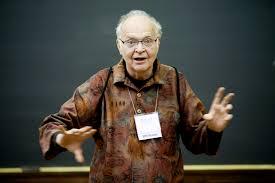
\includegraphics[width=14cm]{../resources/jpg/3.1.algorithms/kunth.jpg}
    \caption*{Dr. Donald Kunth.}
\end{figure}


% ============================= 0011 Algorithm 3116 =================================
\begin{figure}[!h]
    \centering
    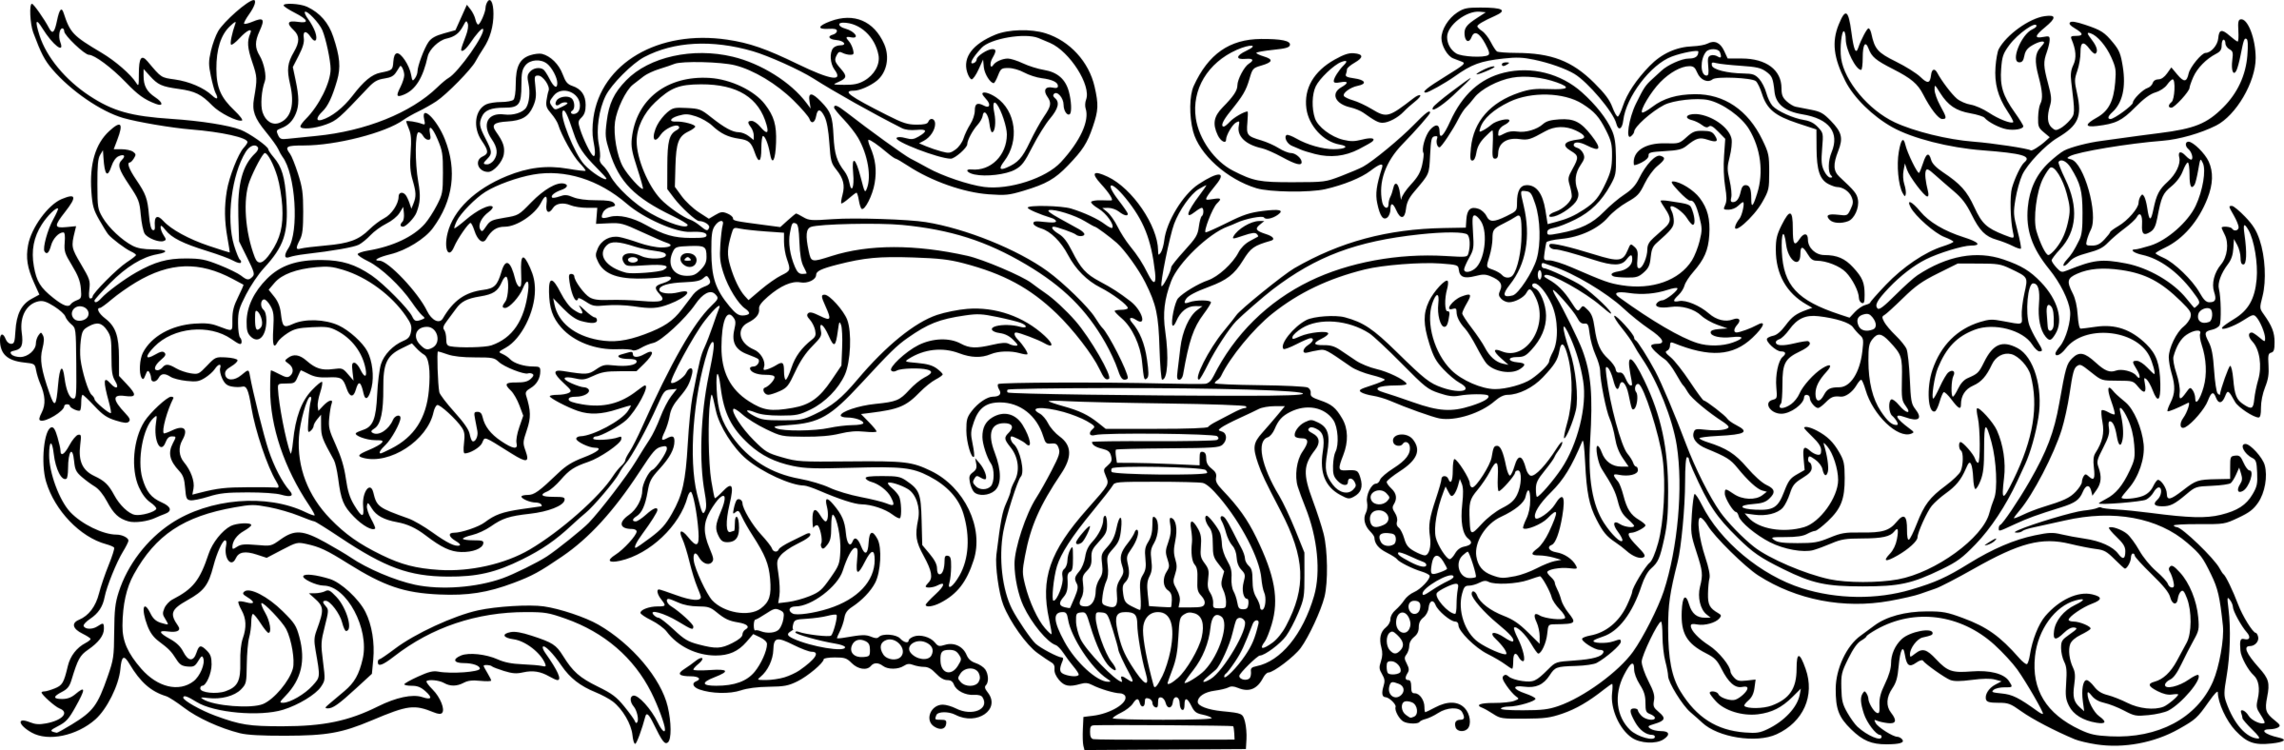
\includegraphics[width=14cm]{../resources/jpg/3.1.algorithms/border1.png}
\end{figure}
\subsection[Find the least element in a sequence.]{
    \color{section} Algorithm 11. \color{black} The least element in a sequence.
}
\vspace{-1\baselineskip}
\documentclass[preview]{standalone}
\usepackage{xcolor}
\usepackage[noend]{algpseudocode}

\begin{document}
		\begin{algorithmic}[0]
			\Statex \color{white} x \color{black}
			\Function{min}{$\rho_1$, $\rho_2$, $\dots$, $\rho_\lambda$: finite sequence of natural numbers}
			\State $\mu \gets \rho_1$
			\For {$\iota = 2, \lambda$}
				\If {$\rho_\iota < \mu$}
					\State $\mu \gets \rho_\iota$
			    \EndIf
			\EndFor
			\State \Return{$\mu$}
			\EndFunction
		\end{algorithmic}
\end{document}

\vspace{1\baselineskip}
\begin{center}
    \lstinputlisting[language=Python, title=\textbf{\color{darkgray}Python}]{../resources/Python/3.1.algorithms/3116.py}
\end{center}
\vspace{1\baselineskip}
\begin{center}
    \lstinputlisting[language=Java, title=\textbf{\color{darkgray}Java}, firstline=11, lastline=20]{../resources/Java/3.1.algorithms/j3116.java}
\end{center}

\end{document}